\documentclass[]{article}
\usepackage{amssymb,latexsym,amsmath}     % Standard packages
\usepackage[pdftex]{graphicx}

\addtolength{\textwidth}{1.0in}
\addtolength{\textheight}{1.00in}
\addtolength{\evensidemargin}{-0.75in}
\addtolength{\oddsidemargin}{-0.75in}
\addtolength{\topmargin}{-.50in}
% \usepackage[lf]{venturis}
\renewcommand{\familydefault}{\sfdefault}  % sans-serif!


\begin{document}

\title{Concept Document}
\author{Team \emph{wut} - Kylar Henderson, Charles Tark,\\ 
Gagik Hakobyan, Julia Cole, Andrew Halpern, Austin Liu}
\maketitle

\section*{High Concept Statement}
You arrive at a dance party fashionably late and realize something is
amuck. All of the other party attendees have been turned into monster
zombies because of the music being played by the evil DJ. You must
withstand hordes of monsters to reach the DJ and save them all with
the power of music.

\section*{Features}
\begin{itemize}
\item 
  Coordinate your actions to the beat of the music
\item 
  Swing a sword
\item 
  Hold up a shield
\item 
  Turn to change direction
\item 
  Cast an Area of Effect attack spell that damages all 
  enemies within a certain number of squares (freezing, blizzard spell)
\item 
  Dance in place to build up “Sync”
\end{itemize}

\section*{Design Goals}
\begin{itemize}
\item
  \textbf{Rhythm Centric Combat} - The goal of the game is to test the
  players’ abilities to follow along with the rhythm of the music. The
  players should feel like they are at a wacky 21st century dance party
  and the combination of techno music and rhythm based combat is geared
  towards a younger audience attracted to electronic dance music.
\item
  \textbf{Play Style} - Players must react quickly to changes in the
  music and the environment around them. The game emphasizes timing
  accuracy, long combo streaks, and short-down time between objectives.
\end{itemize}

\pagebreak
\section*{Market Segment}
\subsection*{Genre}
This is an action rhythm game. The player must defeat enemies by matching your 
actions to the incoming “notes” of the music.

\subsection*{Platform}
Our game is designed for the desktop and will be played with a keyboard. 
It is also recommended that players have headphones for optimal danciness. 

\subsection*{Competition}
\begin{itemize}
\item Dance Dance Revolution (series): This is probably the main
  competition for our game. DDR’s mechanics involve hitting keys to the
  beat of the music and the player must match a specific key pattern to
  progress through the level. In its core, this is one of the main
  mechanics of our game.
\item Guitar Hero (series): Similarly to DDR, Guitar hero involves
  matching a key pattern to the beat of the music, so we again have an
  overlap of mechanics.
\item Crypt of the Necrodancer: To a lesser extent, Crypt of the
  Necrodancer has similar themes. It is a game about fighting monsters
  while confined to a rhythm. However, Crypt of the Necrodancer focuses
  on exploration and Rogue-like elements, while our game focuses on
  combat.
\end{itemize}
\subsection*{Unique Selling Points}
\begin{itemize}
\item Polyrhythms, cross-rhythms (2 on 3, both vertically and
  horizontally) are important to achieving larger boosts - consequently,
  we will try to draw inspiration from world musics that make use of
  this - anything from jazz to sub-saharan African music is fair game.
\item Visual feedback into the game that coordinates with the rhythm
  so that the game could be played on mute in theory.
\item Although it is played like a rhythm game, since it is an
  action-hybrid, elements such as Area of Effect spells bring hectic,
  combat-style gameplay.
\item Certain abilities, such as the Area of Effect spell require the
  use of a certain amount of the “Sync” bar, which doubles as a HP bar.
\end{itemize}

\pagebreak
\section*{Gameplay Sketches}
\begin{figure}[!htb]
\begin{center}
\leavevmode
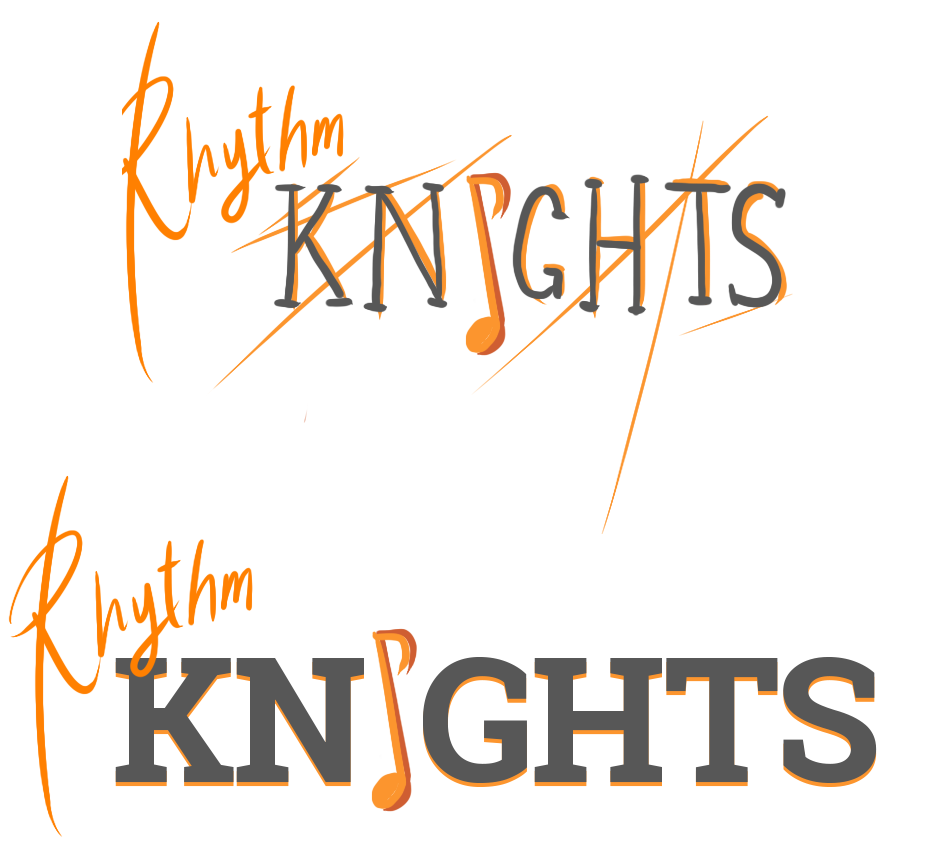
\includegraphics{img/logo.jpg}
\end{center}
\caption{Possible logos for our game, if we continue to use the name 
Rhythm Knights \label{logo}}
\end{figure}

\begin{figure}[!htb]
\begin{center}
\leavevmode
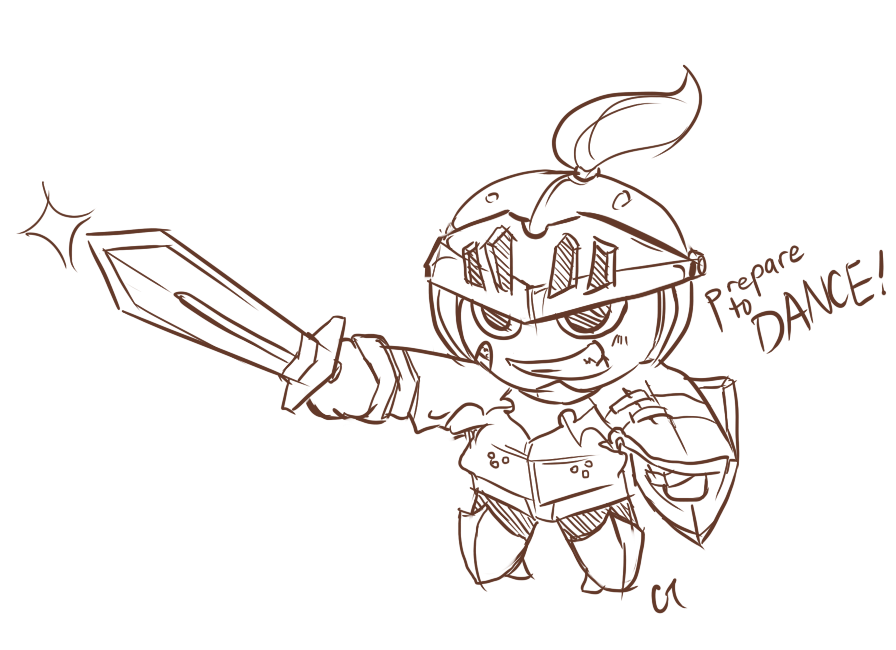
\includegraphics{img/main_char.jpg}
\end{center}
\caption{A sketch of our main character \label{logo}}
\end{figure}


\begin{figure}[!htb]
\begin{center}
\leavevmode
\resizebox{4.7in}{!}{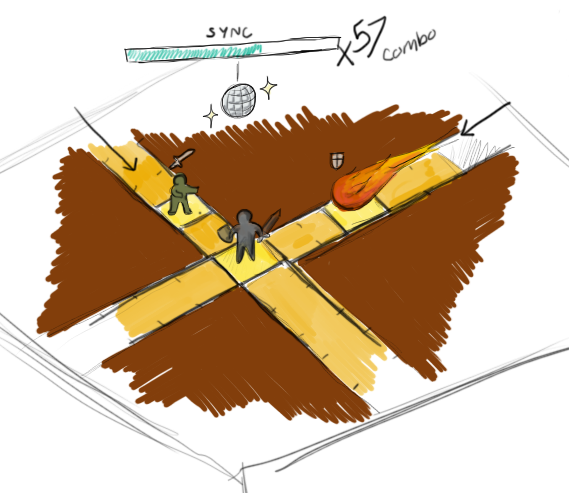
\includegraphics{img/play_sketch.jpg}}
\end{center}
\caption{ This is what we imagine each level will look like. There
will be enemies coming from each of four directions and the player
will have to face the appropriate direction and use the attack shown
above the enemy. There will also by a sync meter at the top of the
screen that shows how well the player is doing\label{play_sketch}}
\end{figure}

\end{document}
